
\chapter{Tubo di risonanza}
\section{Introduzione}
\section{Tubo aperto contenente aria}
Dati geometrici tubo:
lunghezza = $L_{tubo}$ = 90cm
diametro = $d$ = 3.9cm
\\
Data la relazione
\begin{equation} \label{eq:gianni}
\nu_n= \frac{vn}{2L}		
\end{equation}
 con $v$ velocità del suono nel mezzo e $n \in \mathbb{N} = \{1,2,3\dots\}$ 
\\

Verifichiamo che data una certa frequenza $\nu_0$ fondamentale, che viene determinata dal valore $n=1$, quelle successive saranno multipli interi della fondamentale. 



\begin{center}
\begin{tabular}{c|c|c|c|c|c}
$\nu$ (Hz) & 185 & 370 & 558 & 930 & 1320 \\
\midrule
$n$ & 1 & 2 & 3 & 5 & 7\\
\end{tabular}
\end{center}

RIFAI GRAFICO
%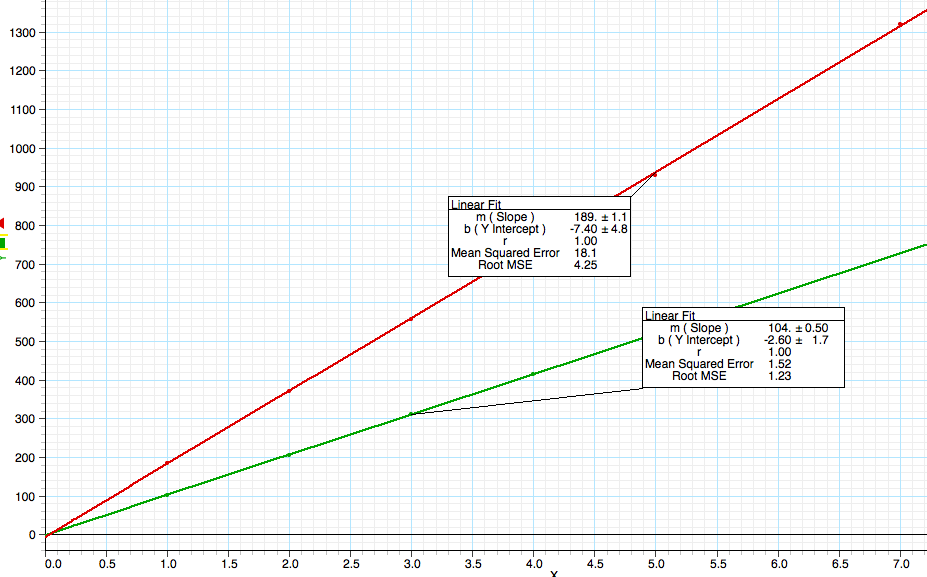
\includegraphics[scale=0.5]{risonanza}

Si verifica sperimentalmente che all'interno di un intervallo minore di 10 Hz lo strumento non è in grado di distinguere ulteriori variazioni nella lettura delle frequenze. Se ne ricava che l'incertezza relativa alle misure è di $\pm$5 Hz.

$$ \frac{v}{2L_{tubo}} = m = \frac{\nu}{n} = (189 \pm 1.1)\ s^{-1}$$

con $m$  coefficente angolare della retta. Per la \ref{eq:gianni} si ha che $\displaystyle{m=\frac{v}{2L}}$, da cui ricaviamo $v$. Prima di confrontare questa formula con i dati sperimentali, però, bisogna apportare una correzione alla formula scritta in precedenza. Per un tubo aperto reale, infatti la posizione di nodi e antinodi dipende anche dal diametro del tubo, pertanto apportiamo la seguente correzione:

$$ L_c = L_{tubo}+0.8d = n\frac{\lambda}{2} $$

dove $d$ è il diametro del tubo (3.9 cm) e $L_{tubo}$ la sua lunghezza. 
Si ricava dunque che $$v=2L_cm=351.994\ m/s$$.
Dunque si vede che:
$$ 2L_c= n.... v = \lambda\nu$$

Si può ricavare $v$ direttamente dalla \ref{eq:gianni} (con la correzione), sostituendo a $\nu$ la frequenza fondamentale $\nu_0 = 185$ Hz

$$ v = 2L_c\frac{\nu}{n} = 344.544\pm9.39\ m/s$$ 
   
 
\subsection{Ventri e nodi}

Posta una frequenza corrispondente a $n>1$, spostiamo all'interno del tubo il microfono e cerchiamo i punti corrispondenti a ventri e nodi (posizione rispetto all'inizio del tubo).\\

\begin{center}
\begin{tabular}{r r r r}

\multicolumn{2}{c}{$\nu$ = 370 Hz}&\multicolumn{2}{c}{$\nu$ = 558 Hz}\\
\textit{nodo 1}:& 0 cm & \textit{nodo 1}:& 0 cm\\
\textit{ventre 1}:& 22.5 cm & \textit{ventre 2}:& 15 cm\\
\textit{nodo 2}:& 45 cm &\textit{nodo 2}:& 30 cm\\
\textit{ventre 2}:& 67.5 cm&\textit{ventre 3}:& 45 cm\\
\textit{nodo 3}:& 90 cm & \textit{nodo 3}:& 60 cm\\
& & \textit{ventre 4}:& 75 cm \\
& & \textit{nodo 4}:& 90 cm \\
\end{tabular}
\end{center}

 
 %propagazione misure
\section{Tubo chiuso ad una estremità, contenente aria}

La condizione per l'instaurarsi di onde stazionarie in un tubo chiuso ad una estremità è data dalla relazione:

\begin{equation}
 L=(2n-1)\frac{\lambda}{4}
\end{equation}

Operativamente, abbiamo risolto l'equazione soprastante rispetto a $n$.

$$ n = \frac{2L_c\nu}{v} + \frac{1}{2} $$

Verifichiamo, come nel caso del tubo aperto, che 

\begin{center}
\begin{tabular}{c|c|c|c|c|c}
$\nu$ (Hz) & 285 & 475 & 670 & 860 & 1050 \\
\midrule
$n$ & 2 & 3 & 4 & 5 & 6 \\
\end{tabular}
\end{center}

\subsection{Ventri e nodi}
$\nu_0$= 475 Hz\\

\begin{center}
\begin{tabular}{r r}
\textit{nodo 1}: & 0 cm\\
\textit{ventre 2}: & 17 cm\\
\textit{nodo 3}: & 34 cm\\
\textit{ventre 4}: & 53 cm\\
\textit{nodo 5}: & 70 cm\\
\end{tabular}

\end{center}

\subsection{Onda quadra}
$t_1 = 185 \mu s $\\
$t_2 = 5160 \mu s $\\
$\Delta t = 4.98*10^{-3}$ s\\
$L = (0.9 - 0.03) m $ (stantuffo 1 cm, microfono 2cm)\\
$v = 349 m/s$

\subsection{Tubo a lunghezza variabile}
Variando la lunghezza del tubo abbiamo cercato la frequenza secondo cui si riusciva a trovare la prima armonica - detto come si sarebe dovuto dire, abbiamo verificat la dipendenza dell'equazione dalla lunghezza del tubo.

\begin{center}
\begin{tabular}{*{5}{c|}c}
L (cm) & 60 & 65 & 70 & 75 & 80 \\
\midrule
$\nu$ (Hz) & 415 & 380 & bianchetto & 340 & 315\\
\end{tabular}
\end{center}


\section{Tubo chiuso da ambo i lati, contenente Kripton}

$L_{tubo}$ = 147 cm\\
$D_{tubo}$ = sacchi cm
$\nu$ = 75.7 Hz
 


\begin{center}
\begin{tabular}{c|c|c|c|c|c}
$\nu$ (Hz) & 102 & 204 & 312 & 415 & 518 \\
\midrule
$n$ & 1 & 2 & 3 & 4 & 5\\
\end{tabular}
\end{center}

Interpolando i dati tramite la funzione lineare 7.1 (con correzione) otteniamo:

$$ m_2 = 104 \pm 0.5 $$ 
\\
Da questa $m$, tramite il procedimento illustrato in precedenza, calcoliamo: 
$$v = 308.4\pm0.5*..  m/s $$
\\
La seguente relazione:
$$v=\sqrt{\frac{\gamma RT}{M}}$$

con $\gamma = \frac{C_p}{C_v}$, $R$ è la costante dei gas, $M$ la massa molare e $T$ la temperatura in gradi Kelvin, ci fornisce il valore teorico della velocità di propagazione di un'onda sonora in relazione alle caratteristiche del mezzo. 
Il risultato atteso è dunque $v=222.7 m/s$. Confrontando questo risultato con il valore misurato sperimentalmente siamo giunti alla conclusione che all'interno del tubo non era presente solo Kripton ma anche una certa percentuale di aria.

\subsection{Onda quadra}
$t_1 = 4.96 ms $\\
$t_2 = 14.6 ms $\\
$\Delta t = 9.64 ms $ \\
Applicando la formula [ref] con $L_{tubo} = 147 cm$, otteniamo:
$$ v = 305.0 \pm \sigma m/s $$ 


